\documentclass[11pt,sort&compress]{elsarticle}

\journal{}
\raggedbottom

\usepackage{amsmath}
\usepackage{lipsum}
\usepackage{amsfonts}
\usepackage{graphicx}
\usepackage{xspace}
\usepackage{epsf}
\usepackage{setspace}
\usepackage{float}
\usepackage[mediumspace,mediumqspace,squaren]{SIunits}
\usepackage{enumerate}
\usepackage{enumitem}
\usepackage{microtype}
\usepackage[margin=1in]{geometry}

\usepackage[]{xcolor}
\usepackage{bm}
\newcommand{\ve}[1]{\bm{#1}}

\newcommand{\ba}{\ve{a}}
\newcommand{\bb}{\ve{b}}
\newcommand{\bu}{\ve{u}}
\newcommand{\bv}{\ve{v}}
\newcommand{\br}{\ve{r}}
\newcommand{\bp}{\ve{p}}
\newcommand{\bt}{\ve{t}}
\newcommand{\bn}{\ve{n}}
\newcommand{\bc}{\ve{c}}
\newcommand{\bq}{\ve{q}}
\newcommand{\bff}{\ve{f}}
\newcommand{\bw}{\ve{w}}
\newcommand{\by}{\ve{y}}
\newcommand{\bx}{\ve{x}}
\newcommand{\be}{\ve{e}}
\newcommand{\bg}{\ve{g}}
\newcommand{\bh}{\ve{h}}
\newcommand{\bs}{\ve{s}}
\newcommand{\bk}{\ve{k}}

\newcommand{\bA}{\ve{A}}
\newcommand{\bD}{\ve{D}}
\newcommand{\bJ}{\ve{J}}
\newcommand{\bS}{\ve{S}}
\newcommand{\bB}{\ve{B}}
\newcommand{\bU}{\ve{U}}
\newcommand{\bV}{\ve{V}}
\newcommand{\bW}{\ve{W}}
\newcommand{\bE}{\ve{E}}
\newcommand{\bQ}{\ve{Q}}
\newcommand{\bP}{\ve{P}}
\newcommand{\bGG}{\ve{G}}
\newcommand{\bRR}{\ve{R}}
\newcommand{\bX}{\ve{X}}
\newcommand{\bM}{\ve{M}}
\newcommand{\bC}{\ve{C}}
\newcommand{\bF}{\ve{F}}
\newcommand{\bI}{\ve{I}}
\newcommand{\bL}{\ve{L}}
\newcommand{\bR}{\ve{R}}

\newcommand{\tn}{\tilde{n}}

\newcommand{\cM}{\mathcal{M}}

\newcommand{\dd}{\text{d}}
\newcommand{\ddd}{\dd R \dd \dot{R}}
\newcommand{\bbE}{\mathbb{E}}
\newcommand{\Rdot}{\dot{R}}
\newcommand{\Rddot}{\ddot{R}}

\newcommand{\muR}{\mu_R}
\newcommand{\muRdot}{\mu_{\dot{R}}}
\newcommand{\sigmaR}{\sigma_R}
\newcommand{\sigmaRdot}{\sigma_{\dot{R}}}

\newcommand{\bmu}{\vec{\boldsymbol{\mu}}}
\newcommand{\btheta}{\vec{\boldsymbol{\theta}}}

\newcommand{\brho}{\boldsymbol{\rho}}
\newcommand{\bLambda}{\boldsymbol{\Lambda}}
\newcommand{\blambda}{\boldsymbol{\lambda}}
\newcommand{\bSigma}{\boldsymbol{\Sigma}}
\newcommand{\bEps}{\boldsymbol{\varepsilon}}
\newcommand{\beps}{\boldsymbol{\varepsilon}}
\newcommand{\bxi}{\boldsymbol{\xi}}
\newcommand{\balpha}{\boldsymbol{\alpha}}
\newcommand{\heps}{\hat{\varepsilon}}
\newcommand{\bdelta}{\boldsymbol{\delta}}
\newcommand{\vblambda}{\vec{\boldsymbol{\lambda}}}
\newcommand{\vbsigma}{\vec{\boldsymbol{\sigma}}}
\newcommand{\vbEps}{\vec{\boldsymbol{\varepsilon}}}
\newcommand{\vbdelta}{\vec{\boldsymbol{\delta}}}
\newcommand{\eps}{\varepsilon}

\newcommand{\vq}{\vec{q}}

\newcommand{\vba}{\vec{\ve{a}}}
\newcommand{\vbu}{\vec{\ve{u}}}
\newcommand{\vbx}{\vec{\ve{x}}}
\newcommand{\vby}{\vec{\ve{y}}}
\newcommand{\vbm}{\vec{\ve{M}}}
\newcommand{\vbmm}{\vec{\ve{m}}}
\newcommand{\vbv}{\vec{\ve{v}}}
\newcommand{\vbh}{\vec{\ve{h}}}
\newcommand{\vbbh}{\vec{\bar{\ve{h}}}}
\newcommand{\vbs}{\vec{\ve{s}}}
\newcommand{\vbF}{\vec{\ve{F}}}
\newcommand{\vbg}{\vec{\ve{g}}}
\newcommand{\vbq}{\vec{\ve{q}}}
\newcommand{\vbr}{\vec{\ve{r}}}

\newcommand{\hx}{\hat{x}}
\newcommand{\hy}{\hat{y}}
\newcommand{\hz}{\hat{z}}

\newcommand{\hbx}{\hat{\ve{x}}}
\newcommand{\hby}{\hat{\ve{y}}}
\newcommand{\hbz}{\hat{\ve{z}}}

\newcommand{\hbF}{\widehat{\ve{F}}}
\newcommand{\hbq}{\widehat{\ve{q}}}
\newcommand{\hbg}{\widehat{\ve{g}}}
\newcommand{\hw}{\widehat{w}}

\newcommand{\hR}{\widehat{R}}
\newcommand{\hRdot}{\widehat{\dot{R}}}

\newcommand{\trho}{\widetilde{\rho}}
\newcommand{\tbrho}{\widetilde{\boldsymbol{\rho}}}
\newcommand{\tx}{\widetilde{x}}
\newcommand{\tbx}{\widetilde{\ve{x}}}
\newcommand{\tbB}{\widetilde{\ve{B}}}

\newcommand{\mom}{\mu}
\newcommand{\bmom}{\boldsymbol{\mu}}
\newcommand{\vbmom}{\vec{\bmom}}
\newcommand{\hbmom}{\widehat{\bmom}}


\newcommand{\EV}{\mathbb{E}}

\newcommand{\dt}{\Delta \tau}
\newcommand{\gdot}{\dot\gamma}

\newcommand\Rey{\mbox{\text{Re}}\xspace}

\newcommand{\cD}{\mathcal{D}}
\newcommand{\cI}{\mathcal{I}}
\newcommand{\cG}{\mathcal{G}}
\newcommand{\cC}{\mathcal{C}}
\newcommand{\cL}{\mathcal{L}}
\newcommand{\dL}{\mathbf{L}}
\newcommand{\dW}{\mathbf{W}}
\newcommand{\dO}{\mathbf{O}}
\newcommand{\dM}{\mathbf{M}}
\newcommand{\dU}{\mathbf{U}}
\newcommand{\dD}{\mathbf{D}}

\newcommand{\cbL}{\overline{\mathcal{L}}}
\newcommand{\baru}{\bar{u}}
\newcommand{\barc}{\bar{c}}
\newcommand{\bars}{\bar{s}}

\newcommand{\bbarf}{\bar{\ve{f}}}
\newcommand{\barbu}{\bar{\ve{u}}}

\definecolor{lightblue}{rgb}{0.63, 0.74, 0.78}
\definecolor{seagreen}{rgb}{0.18, 0.42, 0.41}
\definecolor{orange}{rgb}{0.85, 0.55, 0.13}
\definecolor{silver}{rgb}{0.69, 0.67, 0.66}
\definecolor{rust}{rgb}{0.72, 0.26, 0.06}
\definecolor{purp}{RGB}{68, 14, 156}

\colorlet{lightrust}{rust!50!white}
\colorlet{lightorange}{orange!25!white}
\colorlet{lightlightblue}{lightblue}
\colorlet{lightsilver}{silver!30!white}
\colorlet{darkorange}{orange!75!black}
\colorlet{darksilver}{silver!65!black}
\colorlet{darklightblue}{lightblue!65!black}
\colorlet{darkrust}{rust!85!black}
\colorlet{darkseagreen}{seagreen!85!black}




\usepackage{hyperref}
\hypersetup{
  colorlinks=true,
}

\usepackage[labelfont=bf,font=small]{caption}

\setlength{\parskip}{5pt}
\setlength{\parindent}{0pt}

\usepackage{cleveref}
\usepackage{parskip}

\newcommand{\spencer}[1]{\textcolor{seagreen}{[[Spencer says: #1]]}}


\begin{document}

\hypersetup{
  linkcolor=darkrust,
  citecolor=seagreen,
  urlcolor=darkrust,
  pdfauthor=author,
}

\begin{frontmatter}

\title{{\large\bfseries This is an example document showing how to make a nice looking \\ paper with different \LaTeX commands and packages}}

\author[1]{\vspace{-3ex}Your Name}
\author[2]{Spencer H.\ Bryngelson}
\ead{shb@gatech.edu}

\address[1]{Some other School, Georgia Institute of Technology, Atlanta, GA 30332, USA}
\address[2]{School of Computational Science \& Engineering, Georgia Institute of Technology, Atlanta, GA 30332, USA}


\date{January 1, 2032}

\begin{abstract}
Abstract here
\end{abstract}

\begin{keyword}
   Keywords; Here 
\end{keyword}

\end{frontmatter}

\section{Introduction}

Well-established equations describe even the most complicated flow physics.
Still, full-resolution simulations of them stretch computational resources. 
Reduced-complexity surrogate models are a successful approach to reducing these costs.
Historically, physical insight and analytical techniques have been used to develop these models, including the RANS closure models~\citep{tennekes1972first}.
However, data-driven approaches are emerging as semi-automated tools to accomplish the same task.
Some approaches attempt to represent the time evolution of the physical system via neural networks, a formidable task that involves reducing the entire Navier--Stokes operator~\citep{li2020fourier,lu2021learning}.
An alternative approach is to compute effective equations that act on spatial or temporal averages. 
The governing equations are projected into the reduced or averaged space, and a forcing function is applied to examine the effect of the underlying fluctuations on the averaged behavior. 
~\citet{kraichnan1987eddy} and~\citet{hamba1995analysis} examined Green's function solutions (i.e., using Dirac-delta-function-type forcing) to scalar and momentum transport equations to develop exact expressions for closure operators. 
Similarly, the macroscopic forcing method (MFM) of~\citet{maniMacroscopicForcingMethod2021} quantifies closure operators exactly by examining forcing and averaged responses, called input--output pairs. 
However, as a linear-algebra-based technique, MFM does not require the use Dirac delta functions as forcing basis functions, and others like polynomials~\citep{liu21} and harmonic functions~\citep{shirian22}, can be used. 

We use this approach to accelerate the MFM to create the \textit{Fast MFM}. 
The Fast MFM reveals the locality of the physical models to reduce the sample complexity of standard MFM operator recovery.
We apply Fast MFM to inhomogeneous and turbulent problems and reconstruct the RANS closure operators. 
Specifically, we consider passive scalar transport in a laminar 2D channel flow following \citet{maniMacroscopicForcingMethod2021} and reconstruct the corresponding eddy diffusivity operator, and momentum transport in a canonical turbulent 3D channel flow at $\Rey_\tau = 180$ following \citet{hamba2005nonlocal} and \citet{park21} and reconstruct the corresponding eddy viscosity operator.
These examples display sufficient spatio-temporal richness in their dynamics to argue that the Fast MFM can be applied more broadly. 
For example, one could tackle the open closure problems associated with multiphase flows~\citep{bryngelson19,bryngelson19_ML,vie2016particle,ma2016using}, though we do not address such extensions here.

We briefly introduce MFM and similar approaches for recovering turbulence closure operators in \cref{s:mfm}.
Results are presented in \cref{s:results}, focusing on the 2D and 3D problems analyzed by \citet{maniMacroscopicForcingMethod2021} and \citet{park21}.
\Cref{s:conclusions} discusses the outlook of sparse reconstruction methods like the one presented for other flow problems and PDEs broadly.

\section{Background on the Macroscopic Forcing Method (MFM)}\label{s:mfm}

\subsection{The macroscopic forcing method}

Given a set of linear microscopic equations,
\begin{gather}
    \cL c = s,
    \label{e:micro}
\end{gather}
and an averaging operator $(s, c) \mapsto (\bars, \barc)$, the macroscopic (averaged) operator $\cbL$ is defined to satisfy, for all microscopic solutions $c, s$ of \eqref{e:micro}, 
\begin{gather}
    \cbL \barc = \bars.
    \label{e:macro}
\end{gather}
Often, \eqref{e:micro} are advection-diffusion equations for scalar transport or linearizations of nonlinear PDEs such as Navier--Stokes equations, so the averaging operation can be written as 
\begin{gather}
    \bars = \frac{1}{L_2 \cdots L_{N_d}}\int_{\Omega_{2}} \cdots \int_{\Omega_{N_d}} s(x_1, \ldots x_{N_d}) \, \dd x_2 \cdots \dd x_{N_d},
\end{gather}
where 
\begin{gather}
    \Omega = \Omega_{1} \times \Omega_{2} \times \cdots \times \Omega_{N_d}
\end{gather}
is the physical (possibly spatio-temporal) domain and $L_i$ are the lengths in each coordinate direction $x_i$, $i \in \{1,\dots,N_d\}$.
In this example, the averaged \eqref{e:macro} is a univariate problem in the non-averaged coordinate $x_1$. 
However, we point out that the techniques outlined in this work apply to a wider range of possible averaging operations.

\begin{figure}[H]
    \centering
    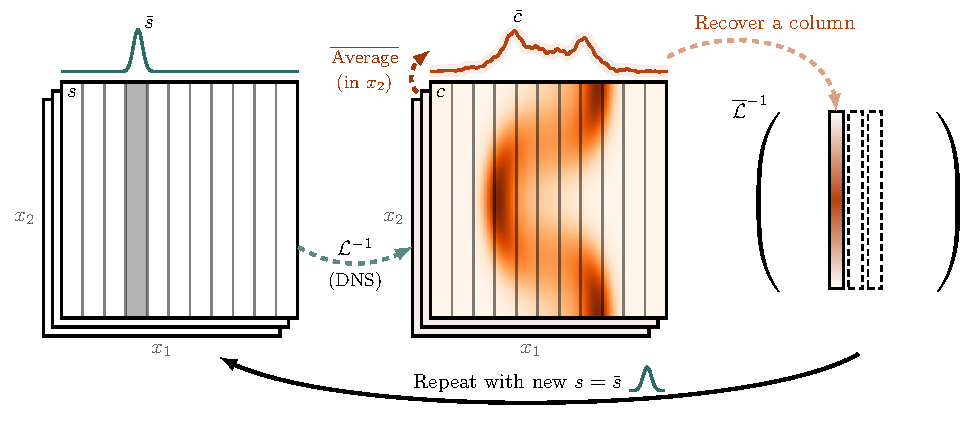
\includegraphics[scale=1]{figures/overview.pdf}
    \caption{
        Schematic of the MFM. 
    }
    \label{f:overview}
\end{figure}

Using MFM, one can determine the exact linear operator $\cbL$ that acts on averages of flow statistics~\citep{maniMacroscopicForcingMethod2021}.
They infer this operator by generating solution pairs to $\cbL \barc = \bars$, obtained from solving the microscopic equations with forcing $\bars$ and macroscopic solution average $\barc$.

\Cref{f:overview} show an example MFM procedure schematically for a two-dimensional problem with coordinate directions $x_1$ and $x_2$.
The relevant averaging direction is $x_2$, with averaged ``strips'' indicating averaging.
This solution is forced by a field $s(x_1,x_2)$ as a Dirac delta function  at a specific $x_1$ coordinate equivalent to its averaged field $\bars(x_1)$.
The inverse solution operator $\cL^{-1}$ solves the problem \eqref{e:micro} for $c(x_1,x_2)$ given $\bars(x_1)$.
This is computationally equivalent to solving the full-resolution system \eqref{e:micro} or DNS.
The averaged solution field $\barc(x_1)$ corresponds to a column (``recover a column'') of a macroscopic solution operator $\cbL^{-1}$ under this averaging scheme.
This procedure is repeated for all non-averaged degrees of freedom.

\begin{figure}
    \centering
    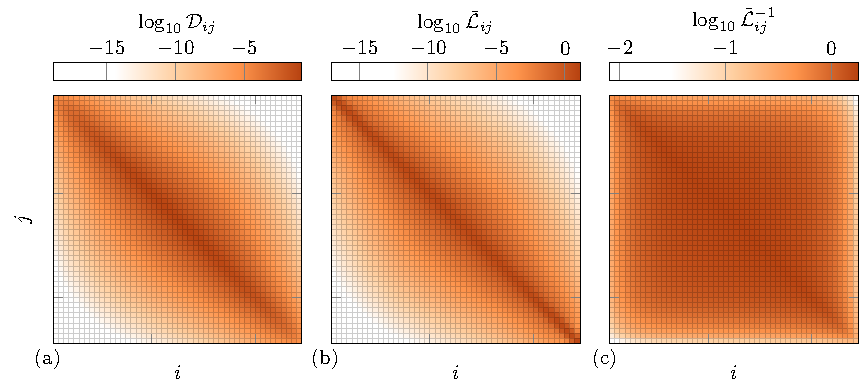
\includegraphics{figures/matrices.pdf}
    \caption{
        Matrices $\cD$, $\cbL$, and $\cbL^{-1}$ as labeled for the 2D channel flow case with 50 non-averaged grid points (and so each is $50 \times 50$) for illustration purposes.
        The inverse operator matrix of (c) is nearly dense, though (a) and (b) are more strongly banded.
        Similar behavior is observed for finer discretizations, which correspond to larger matrices.
    } 
    \label{fig:mfmeddy}
\end{figure}

\begin{figure}
    \centering
    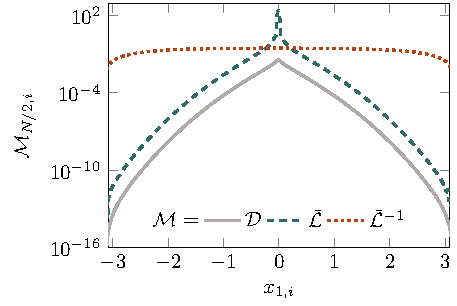
\includegraphics{figures/slices.pdf}
    \caption{
        The middle row of the matrices of \cref{fig:mfmeddy} on a log scale.
        $\cD$ and $\cbL$ have a similar degree of locality, with entries decreasing in magnitude algebraically from the diagonal.
        The discretized operator $\cbL^{-1}$ is dense; along its diagonal entries only decay modestly at the boundaries.
    } 
    \label{fig:slices}
\end{figure}


\subsection{Adaptation to Fast MFM} 

The eddy diffusivity operator is not a divergence-form elliptic solution operator. 
In particular, it is not symmetric. 
Instead of the Cholesky recovery of \citet{schaferSparseRecoveryElliptic2021}, we use an LU recovery that recovers a sparse LU factorization of the target matrix. 
Columns of $\mathrm{L}$ are recovered from matrix--vector products, and rows of $\mathrm{U}$ are recovered from matrix-transpose--vector products (transpose--vector products), which can be computed by solving the adjoint equation of $\cL$.
No rigorous guarantees exist for the accuracy of LU reconstruction applied to eddy diffusivity matrices.
However, \citet{schafer2017compression} show a wide range of diffusion-like operators, including those produced by fractional-order Mat{\'e}rn or Cauchy kernels, produce sparse Cholesky factors, despite the lack of theory supporting this observation.

\subsection{Fast MFM on nonsymmetric operators}\label{s:fmfm}
As remarked by \citet{schaferSparseRecoveryElliptic2021}, a LU version of Cholesky reconstruction that extends to nonsymmetric matrices requires not only matrix--vector products but also transpose--vector products.
Similar requirements arise in hierarchical low-rank approaches~\citep{halko2011finding,lin2011fast}. 
Schur complementation commutes with transposition, in the sense that
\begin{gather}
    \left(\cbL\right)^{\top}
    =
    \left(\left(\cL^{-\top}\right)_{1, 1}\right)^{-1}
    =
    \left(\cL^{\top}\right)_{1, 1} - \left(\cL^{\top}\right)_{1, 2} \left(\left(\cL^\top\right)_{2,2}\right)^{-1} \left(\cL^\top\right)_{2 ,1} .
    \label{eqn:mfm_schur_transpose}
\end{gather}
As a result, transpose--vector products with $\cbL$ can be obtained by applying (inverse or forward) MFM to the $\cbL^{\top}$.
Here $x$ is the spatial coordinate, and $t$ denotes time.
The resulting PDE is often called the adjoint problem and frequently arises in the computation of sensitivities of solutions of PDEs with respect to their coefficients, boundary, and initial conditions.
We empirically validate our method using matrix--vector products and transpose--vector products obtained from a full eddy diffusivity operator constructed via brute force (column-by-column) MFM. 
We leave an adjoint-based MFM that efficiently implements transpose--vector products as future work.

\section{Results}\label{s:results}

\subsection{Steady-state laminar channel flow}

Consider a 2D domain representing a channel with left and right walls at $x_1 = \pm \pi$ with Dirichlet boundary condition $c = 0$ and the top and bottom walls with $x_2 = 0,2\pi$ with no flux condition $\partial c/\partial x_2 = 0$.
The scalar field $c(x_1,x_2)$ is governed by a steady advection--diffusion equation with a uniform source term
\begin{gather}
    u_1 \frac{\partial c}{\partial x_1} + u_2 \frac{\partial c}{\partial x_2} = 0.05 \frac{\partial^2 c}{\partial x_1^2} + \frac{\partial^2 c}{\partial x_2^2} + 1,
\end{gather}
where the unequal diffusion constants in the coordinate directions are an outcome of directional nondimensionalization.
The flow is incompressible and satisfies no-penetration boundary conditions on the walls. 
The steady velocity field is prescribed as
\begin{gather}
    u_1 = (1 + \cos(2 x_1))\cos(2 x_2), \quad u_2 =\sin(2 x_1)\sin(2 x_2).
\end{gather}
The PDE is discretized on a uniform staggered mesh with $N_1$ and $N_2 = N_1/2$ grid points in the $x_1$ and $x_2$ coordinate directions. 
Second-order accurate central differences are used. 
The advective fluxes at the cell faces are computed via second-order interpolation and then multiplication of the divergence-free velocity at the face centers.
At the cell faces $x_1=\pm \pi$, the fluxes are computed using ghost points that enforce the specified Dirichlet boundary conditions, while at the cell faces at the top and bottom boundaries, the no flux condition is naturally enforced. 

\begin{figure}
    \centering
    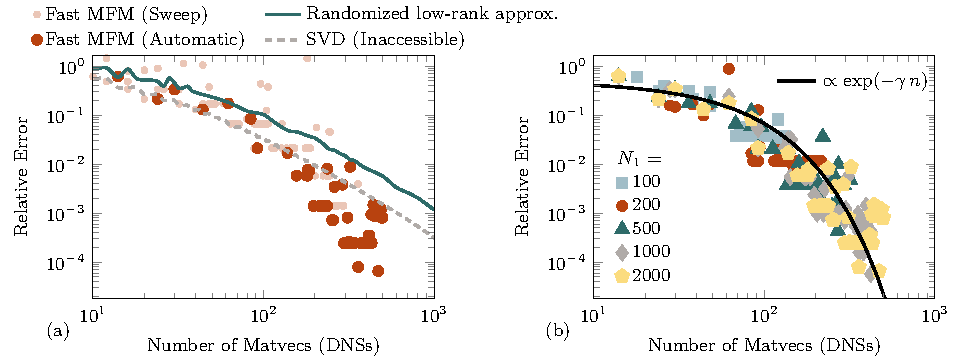
\includegraphics[scale=1]{figures/err-peel-laminar.pdf}
    \caption{
        Relative $L_2$ errors between the exact MFM operator $\cD$ and its reconstruction for the laminar flow configuration.
        In (b), only the Fast MFM with automatically chosen parameterization is shown, but for different resolutions $N_1$ and the number of matrix--vector products is denoted by $n$ in the legend.
    }
    \label{f:error_peeeling_lam}
\end{figure}

\Cref{f:error_peeeling_lam} shows the macroscopic operator errors for the laminar flow configuration.
In (a), the mesh resolution in the $x_1$ (non-averaged) coordinate is $N_1 = 2000$.
Fast MFM errors are smaller than a truncated SVD reconstruction of the same operator. 
The latter provides the optimal low-rank approximation of $\cD$ but requires access to the full operator and is, therefore, not practical.
A randomized low-rank representation is also shown, which is available.
The errors for this reconstruction are about $10$ times larger than the SVD.
Compared to Fast MFM, these errors are also larger as the number of matrix--vector products increases.
The Fast MFM requires choosing the distance between basis functions of the same color and the level at which the wavelet coefficients are truncated. 
The former parameter dictates the cost-accuracy trade-off, and choosing a suitable truncation can improve the method's cost and stability.
A sweep over a wide range of parameters is shown in shaded markers.
We use a heuristic to set these parameters, which results in the non-shaded darker marks. 
Sometimes, the heuristic still produces poor parameter choices resulting in larger Fast MFM errors.

In \cref{f:error_peeeling_lam}~(b), we perform a similar analysis but only show the Fast MFM results for varying mesh sizes $N_1$.
Errors decrease exponentially with the number of matrix--vector products (corresponding to the number of DNSs) with about the same fit coefficients regardless of $N_1$.
This indicates that the Fast MFM reconstruction is dependent on the \textit{physical locality} of the operator, not a numerical or discretized one. 
Thus, operator recovery for high-resolution simulations has an out-sized benefit over traditional MFM. 

\begin{figure}
    \centering
    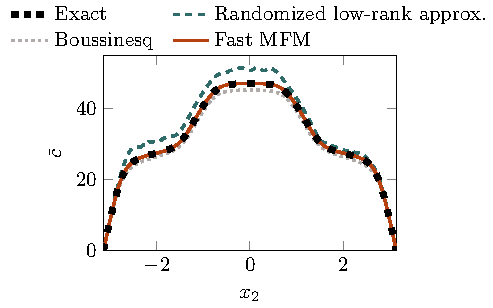
\includegraphics[scale=1]{figures/laminar-reconstructions.pdf}
    \caption{
        Reconstruction of $\barc$ for the laminar, steady channel flow problem. 
        Results are shown for a randomized low-rank approximation, the Boussinesq approximation, and the Fast MFM result. 
        This visualization is 26 out of 2000 possible samples.
    }
    \label{f:lam-reconstructions}
\end{figure}

\Cref{f:lam-reconstructions} shows the application of the recovered operator of \cref{f:error_peeeling_lam} to compute $\barc$. 
The exact result is computed using $N_1 = 2000$ DNSs to recover $\barc$.
For fewer DNSs, $26$ out of the $2000$ total non-averaged degrees of freedom, the Fast MFM result matches the exact result well, but the other methods do not. 
The Boussinesq approximation is purely local~\citep{hamba2004nonlocal}:
\begin{gather}
    -\overline{u_1'c'} = D_{\mathrm{Boussinesq}}\frac{\partial \bar{c}}{\partial x_1},
\end{gather}
where
\begin{gather}
    D_{\mathrm{Boussinesq}}(x_1) = 
    \int_{y_1} \cD(x_1,y_1) \dd y_1.
\end{gather}

\subsection{Turbulent channel flow}

We next consider a fully-developed turbulent channel flow, reconstructing eddy diffusivities, which, for momentum transport, are commonly referred to as eddy viscosities.
The incompressible Navier--Stokes equations are
\begin{gather}
    \frac{ \partial u_i}{\partial t} + 
    \frac{\partial u_j u_i}{\partial x_j} = 
    -\frac{\partial p}{\partial x_i} + 
    \frac{1}{\Rey} \frac{\partial^2 u_i}{\partial x_j \partial x_j} + r_i, \\
    \frac{\partial u_j}{\partial x_j} = 0,
\end{gather}
where $\br$ is a body force, $p$ is the pressure, and $\bu$ are velocities.
Following \citet{maniMacroscopicForcingMethod2021}, the generalized momentum transport equation associated with MFM for a computed $u_i$ field is
\begin{gather}
    \frac{ \partial v_i}{\partial t} + 
    \frac{\partial u_j v_i}{\partial x_j} = 
    -\frac{\partial q}{\partial x_i} + 
    \frac{1}{\Rey} \frac{\partial^2 v_i}{\partial x_j \partial x_j} + s_i, \\
    \frac{\partial v_j}{\partial x_j} = 0,
\end{gather}
for a pressure-like term $q$ that ensures incompressibility. 

\begin{figure}
    \centering
    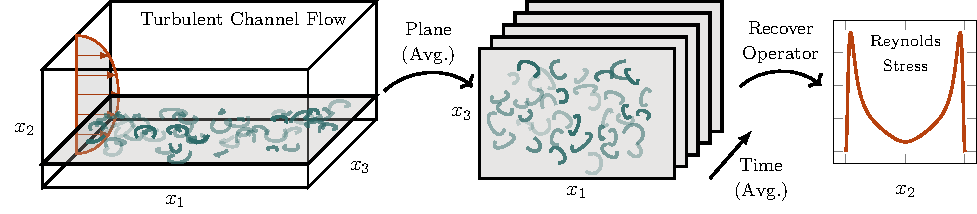
\includegraphics[scale=1]{figures/3d-channel.pdf}
    \caption{
        Diagram of the Fast MFM reconstruction procedure for the 3D turbulent channel flow case.
    }
    \label{f:schematic-turb}
\end{figure}

We consider a case with $\Rey_\tau = u_\tau \delta / \nu = 180$ where $\delta$ is the channel half-width and $u_\tau$ is the friction velocity.
The mean flow is in the $x_1$ direction, the $x_2$ direction is wall-normal, and the $x_3$ direction is the span with periodic boundaries.
The streamwise domain length is $2\pi$, and the spanwise length is $\pi$.
The body force, $\br$, is the mean pressure gradient in the periodic simulation and is $\br=(1,0,0)$ in this nondimensionalized problem. 
The incompressible Navier--Stokes equations are solved using direct numerical simulation with a $144^3$ grid for $T = 500 \delta/u_\tau$ to ensure statistical convergence.
Simulation-result baselines, including the discretized $\cD$ and $\cL$ matrices, for this case follow from \citet{park21} and are used herein.
\Cref{f:schematic-turb} shows our MFM procedure, averaging all independent variables except for the wall-normal coordinate $x_2$.
We thus recover the Reynolds stresses as a function of $x_2$. The generalized eddy viscosity is given by
\begin{gather}
    - \overline{ u_\beta^\prime u_\gamma^\prime } (\bx) = 
    \int_{\by} \cD^{(\beta\gamma)} (\bx,\by)
    \frac{ \partial \bar{u}_1}{\partial x_2} {\bigg|}_{\by} \dd \by
\end{gather}
where $\cD^{\beta\gamma}$ in our notation represents $\cD_{\beta\gamma21}$ in traditional notation for the eddy viscosity tensor \cite{hamba2005nonlocal}.

\begin{figure}
    \centering
    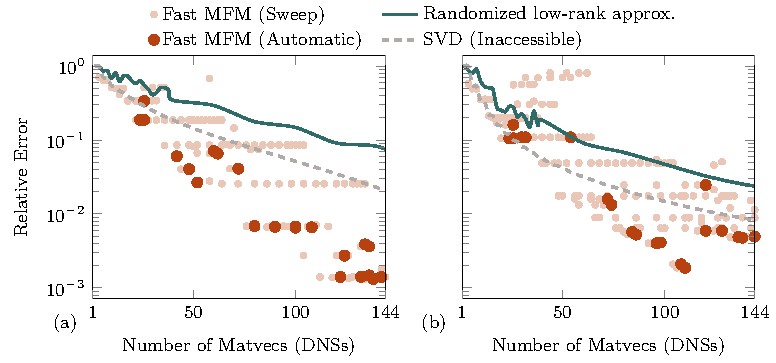
\includegraphics[scale=1]{figures/err-peel-turbulent.pdf}
    \caption{
        Relative errors in the recovered eddy viscosity kernels (a) $\cD^{21}$ and (b) $\cD^{11}$ are shown for the $\Rey_\tau = 180$ turbulent channel flow configuration.
    }
    \label{f:error_peeeling_turb}
\end{figure}

\Cref{f:error_peeeling_turb} shows the errors in the recovered eddy viscosities.
The errors are computed as the difference in operator norms between the approximate and exact solutions to the discretized problem. 
The exact solution is recovered via brute force IMFM, which computes each non-averaged degree of freedom via forcing each $s_i$ independently to recover all columns of $\cD^{\beta\gamma}$  for each $\beta$ and $\gamma$.
In \cref{f:error_peeeling_turb}, the trends of (a) and (b) are similar, with the Fast MFM having smaller errors than both the SVD, which is inaccessible in practice, and a randomized low-rank approximation of it that is accessible.
The differences in errors are small for small numbers of matrix--vector produces as the peeling procedure removes the long-range behaviors.
For larger numbers of matrix--vector products, the difference increases.
Fast MFM has a factor of about 100 smaller errors than the low-rank approximation for 100 matrix--vector products in both (a) and~(b).

\begin{figure}
    \centering
    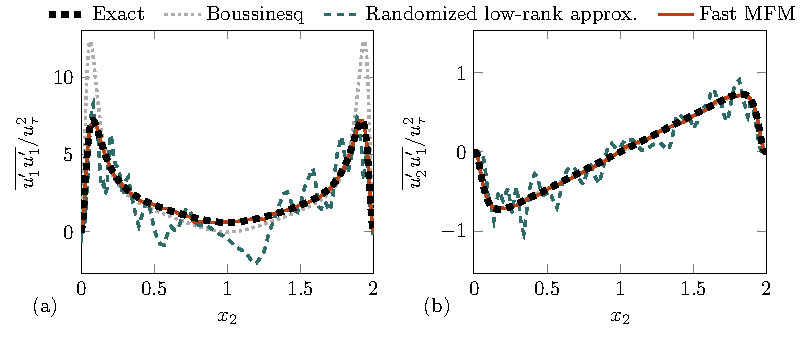
\includegraphics[scale=1]{figures/turbulent-reconstructions.pdf}
    \caption{
        Reynolds stress reconstructions (a) $\overline{u_1^\prime u_1^\prime}$ and (b) $\overline{u_2^\prime u_1^\prime}$ for the turbulent channel flow configuration.
        Results are shown for 20 out of 144 possible samples.
    }
    \label{f:reconstructions}
\end{figure}

\Cref{f:reconstructions} shows the Reynolds stress reconstructions for the turbulent channel flow. 
While direct computation of Reynolds stresses needs only one DNS, we use Reynolds stresses as a metric to assess the accuracy of the recovered eddy viscosity operator, which inevitably requires multiple simulations.
The Fast MFM results (solid, thin line) are compared with the Boussinesq approximation and a randomized low-rank procedure.
Exact results are recovered via brute-force MFM.
For 20 simulations, the difference between the exact solution and Fast MFM is not discernible.
For the same number of simulations, the low-rank procedure does not produce a reasonable approximation for either component.
The Boussinesq approximation is a good one for the transverse stress component $\overline{u_2^\prime u_1^\prime}$ of \cref{f:reconstructions}~(b) but does poorly with the $\overline{u_1^\prime u_1^\prime}$ reconstruction in \cref{f:reconstructions}~(a).

\section{Conclusion}\label{s:conclusions}

This work explores a linear algebra approach to reconstructing closure operators.
Fast MFM uses sparse recovery and peeling techniques, revealing local behaviors that crafted forcings can simultaneously recover.
Results show that tens of simulations are required to reconstruct the eddy diffusivity operator and averaged field to visual accuracy.
This contrasts against brute-force MFM, which forces each degree of freedom and is thus prohibitively expensive; the Boussinesq approximation, which is shown to have inaccuracies in some test cases; randomized low-rank approximations, which, while feasible, have poor accuracy; and even SVD, which performs worse than Fast MFM and is inaccessible in a simulation environment.
While other ongoing work focuses on modeling the nonlocal eddy diffusivity using partial differential equations and limited information about the exact eddy diffusivity, the Fast MFM procedure recovers full nonlocal eddy diffusivity operators at low sample complexity. 
It is a stepping stone toward the long-term goal of sample-efficient recovery of coarse-grained time integrators.

\section*{Acknowledgements}

This work used Bridges2 at the Pittsburgh Supercomputing Center through allocation TG-PHY210084 (PI Spencer Bryngelson) from the Advanced Cyberinfrastructure Coordination Ecosystem: Services \& Support (ACCESS) program, which is supported by National Science Foundation grants \#2138259, \#2138286, \#2138307, \#2137603, and \#2138296.
SHB also acknowledges the resources of the Oak Ridge Leadership Computing Facility at the Oak Ridge National Laboratory, which is supported by the Office of Science of the U.S.\ Department of Energy under Contract No.\ DE-AC05-00OR22725. 
SHB acknowledges support from the Office of the Naval Research under grant N00014-22-1-2519 (PM Dr.\ Julie Young).
FS gratefully acknowledges support from the Office of Naval Research under grant N00014-23-1-2545 (PM Dr.\ Reza Malek-Madani).
JL was supported by the Boeing Company. 
AM was supported by the Office of Naval Research under grant N00013-20-1-2718. 
The authors gratefully acknowledge Danah Park for providing the DNS and MFM data of the turbulent channel flow simulations and Dana Lavacot for fruitful discussions.

\bibliographystyle{model1-num-names}
\bibliography{main.bib}
\end{document}
